\section{Neural Networks}

In this section, I will describe the Progression from Normal Neural network to Recurring Neural Networks - RNN. In the end, I'll show that the GRU works well and I have solved what I set out to do. 


The various results of this research activity will be presented. The results will majorly be training and validation performance. From the above discussion, it should be noticed that GRU is performing extremely better than both feed-forward network and LSTM network.  

\subsection{Training Results}

Training results pertain to how quickly and efficiently a given networks understands and learns its environment. The training efficiency of GRU is depicted in Figure ~\ref{fig:trg}, epoch number vs learning loss. The learning loss drastically decreases right from first epoch. Rapid decline continues until the 40th epoch, then slowly reaches to zero before the 100th epoch. This clearly indicates the superiority of GRU over LSTM and FFNN (feed-forward neural network). This performance clearly hints the best prediction accuracy of GRU.  



\subsection{Validation}

Validation results are also shown in Figure ~\ref{fig:trg}, with x-axis showing the epoch number and y-axis showing the prediction error. 150 epochs have been employed to validate the model. Although validation does not approach to zeros exactly, but such a small error could be acceptable for the estimation of GPV. So, it does validate that GRU can perform the best amongst the class of recurrent neural networks. It looks like the efficient use of long-short memory has outclassed the performance of other networks. 


\subsection{Subsection title}
Neural Networks and more advanced technologies. Right now we use Pandas for everything and it's enough, except when it's not. The more advanced we go into tech, the more basic the Machine Learning tools.

Some Machine Learning models are very dependent on used materials. SCI-KIT uses the most basic of Neural networks. What you'll notice from GPV-Take 1 is that you can't create modern systems with SCI-KIT because it is the highest level of abstraction.

Here, I'll need to show the results of the Google Colab Notebook - Gross Production Value 1 and the abysmal results I got using SCI-KIT

We use SCI-KIT for scaling. It implements it very well. Train - Test - Split
\cite{ponce1989engineering}


\subsubsection{Topology}

In this work, LSTM and GRU variants of recurrent networks have been used as computational machines. The results of these algorithms are compared with a feed-forward network. For all the networks the number of input neurons are three, with 64 hidden neurons and a single output neuron.  

In the feedforward network, 64 neurons are divided equally in 8 consecutive hidden layers. Although the network has become extremely complex, but the complexity remains essentially in vain. The training accuracy and prediction value were found to be poor. 

The structure of LSTM requires that some neurons be assigned to the memory making region, known as cell, which serves the purpose of holding long-term desired information. The training machines can assign different number of neurons to cell memory and to the hidden layer depending upon the user's choice. The decision, taken by the user are dictated by various factors. Larger amount of memory can improve accuracy of prediction hugely, but speed of consecutive predictive operations could be impeded. So, the decision should be taken based on the optimum between speed and accuracy. 

GRU does not require dedicated long-term memory, but it inherits the features of LSTM. It does update the neurons and lets them forget older data in similar fashion to that of LSTM. This algorithm can provide better speed and accuracy management.  

A representative Feed Forward Network is shown in Figure ~\ref{fig:feedforward} showing the resulting graph.

We can conclude that this method will not serve our purpose. 


\begin{figure}[h!]
	\centering
	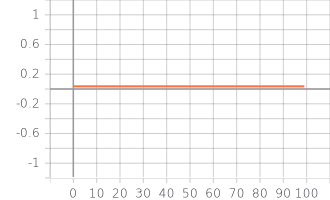
\includegraphics[width=0.35\textwidth]{fig/epoch_accuracy.png}
	\caption{Feed Forward Network}
	\label{fig:feedforward}
\end{figure}



\subsubsection{Model Training}

The models have been trained with extensive number of epochs. The training performance and achieved accuracy are shown in Figure ~\ref{fig:feedforward} and Figure ~\ref{fig:trg} respectively. The x-axis indicates the epoch number, while the y-axis indicates the training loss. From Figure ~\ref{fig:feedforward}, it should be noticed that even with 100 epochs, the performance of feed-forward network could not be improved. So, further analysis of this network is left out. Figure ~\ref{fig:train} indicates the training performance of the proposed RNN’s networks. As the training continues epoch-by-epoch, networks keep on learning the underlying system better and better. So, LSTM indicates some fluctuations, but they can be ignored in comparison to feedforward network. It can clearly be seen that accuracy of LSTM and GRU has surpassed that of feed-forward network. This might have occurred due to foundations of LSTM and GRU on recurrent networks. 

\begin{figure}[h!]
	\centering
	\begin{subfigure}{.5\textwidth}
		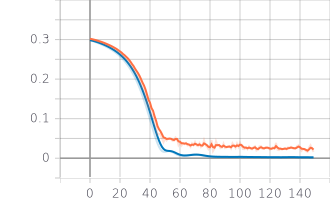
\includegraphics[width=0.35\textwidth]{fig/trg.png}
		\caption{LSTM vs GRU I}
		\label{fig:trg}
	\end{subfigure}%
	\begin{subfigure}{.5\textwidth}
		\centering
		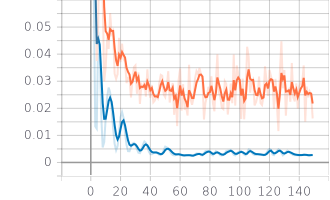
\includegraphics[width=0.35\textwidth]{fig/train.png}
		\caption{LSTM vs GRU II}
		\label{fig:train}
	\end{subfigure}	
	\caption{Training Performance between LSTM and GRU}
\end{figure}

\section{Model GUI}

Abubakar Abid's \cite{abid2019gradio} research highlights the challenge of accessing machine learning models. According to him, the accessibility challenge makes collaboration more difficult. To improve accessibility, he and his team developed Gradio.

Gradio is a Python library that generates an easy-to-use UI for machine learning models. Access to the model is as easy as sharing a URL. This solution was not without its drawbacks. Because this app in still a work-in-progress, the URL is only valid for 6 hours. In order to provide a workaround this problem, i deployed the Gradio UI to Heroku. 